\documentclass{assignment}
\usepackage[pdftex]{graphicx}
\usepackage{xcolor}
\definecolor{LightGray}{gray}{0.95}
\usepackage{fancyvrb, minted}
\usepackage[letterpaper, margin = 2.5cm]{geometry}
\usepackage[T1]{fontenc}
\usepackage{amsmath, amsfonts, amssymb}
\usepackage{hyperref, url} 
\usepackage{fancyhdr}
\usepackage{xcolor}
\usepackage{enumitem}
\newcommand{\R}{\mathbb{R}}
\usepackage{listings}
\definecolor{codegreen}{rgb}{0,0.6,0}
\definecolor{codegray}{rgb}{0.5,0.5,0.5}
\definecolor{codepurple}{rgb}{0.58,0,0.82}
\definecolor{backcolour}{rgb}{0.95,0.95,0.92}



\student{Gabriel Ferreira}   
\semester{Spring 2024}                         
\date{}  

\courselabel{COM S 474/574} 
\exercisesheet{HW3}{Optimization}

\school{Department of Computer Science}
\university{Iowa State University}

\begin{document}

%-----------------------------------------------------------------------------------------------
\begin{problem}
\section{Definifitions}

\subsection{Numbers}
\begin{enumerate}
\item Are the following sets convex?
\begin{enumerate}[label=\alph*)]
    \item \(\{x \mid x \in \R^2,x^Tx \leq2\}\)\\\\
    Yes, this set is convex.\\
    \item \(\{x \mid x \in \R^2,x^Tx \geq 2\}\)\\\\
    Yes, this set is convex.\\
\end{enumerate}
\item Are the following sets strictly convex?
\begin{enumerate}[label=\alph*)]
    \item \(\{x \mid x \in \R^2,x^Tx \leq2\}\)\\\\ No, this set is not strictly convex.\\
    \item \(\{x \mid Ax \leq 0\}\)($A = \begin{bmatrix}
        1&1\\1&-1
    \end{bmatrix}$)\\\\ No, this set is not strictly convex.\\\\
\end{enumerate}

\item Are the following functions convex?
\begin{enumerate}[label=\alph*)]
    \item $f(x) = x^2, x \in \R$\\\\
    Yes, this function is convex.\\
    \item $f(x) = x^2, x \in [0,1]$\\\\
    Yes, this function is convex.\\
    \item $f(x) = x^tx + 4, x \in \R^2$\\\\
    Yes, this function is convex.\\
    \item $f(x) = x^tx + 4, x \in \R^2, x^tx \geq 2$\\\\
    Yes, this function is convex.\\
\end{enumerate}

\item Are the following matrices Positive Definite (PD), Positive Semi-Definite (PSD), Negative Definite (ND), or Negative Semi-Definite (NSD)? Please explain your answers.
\begin{enumerate}[label=\alph*)]
    \item $\begin{bmatrix}
        0&0\\0&4         
    \end{bmatrix}$\\\newline
    This matrix can be interpreted as diagonal matrix. Its eigenvalues, found on the diagonal, are $(\lambda_1 = 0, \lambda_2 = 4)$. \textbf{Since both eigenvalues are non-negatives, the matrix is positive semi-definite (PSD).}\\\\

    \item $\begin{bmatrix}
        1&1\\1&4
    \end{bmatrix}$\\

    $A-I\lambda = \begin{bmatrix}
        1&1\\1&4
    \end{bmatrix} - \begin{bmatrix}
        \lambda&0\\0&\lambda
    \end{bmatrix} = \begin{bmatrix}
        1-\lambda&1\\1&4-\lambda
    \end{bmatrix}$\\

    $\det(A - I\lambda) = (1-\lambda)(4-\lambda)-1$\\
    $\det(A - I\lambda) = 4-5\lambda + \lambda^2 - 1$\\
    $\det(A - I\lambda) = \lambda^2 - 5\lambda + 3 = 0$\\\\

    $\lambda=\frac{-b \pm \sqrt{b^2-4ac}}{2}$\\
    $\lambda=\frac{-(-5) \pm \sqrt{(-5)^2-4 \times1 \times 3}}{2} = $
    $\frac{5 \pm \sqrt{13}}{2}$\\
    $\lambda_1 \approx 4.303$\\
    $\lambda_2 \approx 0.697$\\
    
    \textbf{Given both eigenvalues are positives, this matrix is positive definite (PD).}\\\\

    \item $\begin{bmatrix}
        -5&2&0\\
        2&-3&1\\
        0&1&-2
    \end{bmatrix}$\\

    $A-I\lambda = \begin{bmatrix}
        -5&2&0\\
        2&-3&1\\
        0&1&-2
    \end{bmatrix} - \begin{bmatrix}
        \lambda&0&0\\0&\lambda&0\\0&0&\lambda
    \end{bmatrix} = \begin{bmatrix}
        -5-\lambda&2&0\\2&-3-\lambda&1\\0&1&-2-\lambda
    \end{bmatrix}$\\\\

    $\det(A - I\lambda) = (-5-\lambda)[(-3-\lambda)(-2-\lambda)-1] - 2[2(-2-\lambda)-0]$\\
    $\det(A - I\lambda) = (-5-\lambda)(6+3\lambda+2\lambda+\lambda^2-1) -2(-4-2\lambda)$\\
    $\det(A - I\lambda) = -30-15\lambda-10\lambda-5^2+5-6\lambda-3\lambda^2-2\lambda^2-\lambda^3+\lambda+8+4\lambda$\\
    $\det(A - I\lambda) = -(-\lambda^3 - 10\lambda^2-26\lambda-17)$\\
    $\det(A - I\lambda) = \lambda^3 + 10\lambda^2+26\lambda+17 = 0$
    \\

    $\lambda^3 + 10\lambda^2+26\lambda+17 \div (\lambda + 1)$\\

    After applying synthetic division we have the following:\\
    $(\lambda+1)(\lambda^2+9\lambda+17) = 0$\\
    $\lambda_1 = -1$\\\\
    
    $\lambda=\frac{-9 \pm \sqrt{9^2-4 \times1 \times 17}}{2} = $
    $\frac{-9 \pm \sqrt{13}}{2}$\\
    $\lambda_2 \approx -6.303$\\
    $\lambda_3 \approx -2.697$\\

    \textbf{Given all eigenvalues are negatives, this matrix is negative definite (ND).}\\\\
    
\end{enumerate}

\item Are the following functions Lipschitz continuous? Why?\\\\
$\forall x,y \in \R^n, ||f(x) - f(y)|| \leq L||x-y||$\\\\
A differentiable function is L-Lipschitz if and only if its differential is uniformly bounded by L.
\begin{enumerate}
    \item $f(x) = \sqrt{x},x \in [0,1]$\\\\
    $f'(x) = \frac{1}{2\sqrt{x}}$\\

    This function is \textbf{not} Lipschitz continuous because its derivative $f'(x) = \frac{1}{2\sqrt{x}}$ becomes unbounded as x approaches 0, which breaks the Lipschitz condition that requires the function's differential to be uniformly bounded by L. Therefore, the inequality does not hold in this domain.\\


    \item $f(x) = x^2, x \in \R$\\\\
    $f'(x) = 2x$\\

    This function is \textbf{not} Lipschitz continuous because its derivative $f'(x) = 2x$ becomes unbounded as x tends to infinity or negative infinity, which breaks the Lipschitz condition that requires the function's differential to be uniformly bounded by L. Therefore, the inequality does not hold in this domain.\\

    \item $f(x) = x^2, x \in [0,1]$\\\\
    $f'(x) = 2x$\\

    By restricting the domain of the function to [0,1], it becomes Lipschitz continuous because the derivative, $f'(x) = 2x$ is bounded within this domain. The maximum value of the derivative is 2 ocurring at $x=1$, which allows us to choose $L=2$ as Lipschitz constant. Therefore, the inequality holds in this domain.\\

    \item $f(x) = |x|, x \in \R$\\\\
    When $x>0$:
    $f'(x) = 1$\\

    When $x<0$:
    $f'(x) = -1$\\

    This functions is Lipschitz continuous because its rate of change is bounded across the entire domain $\R$. Although the function is not differentiable at $x=0$, the maximum absolute value of its slope is 1 for both sides of its domain. Therefore, the inequality holds for this function.\\

    \item $f(x) = \sqrt{7x^2 + 4}, x\in\R$\\\\
    $f'(x) = \frac{7x}{\sqrt{7x^2+4}}$\\

    This functions is Lipschitz continuous because its rate of change is bounded across the entire domain $\R$. As x tends to infinity or negative infinity, $f'(x)$ approaches $\sqrt{7}$, which allows us to use it as Lipschitz constant. Therefore, the inequality holds for this function.\\

    \item $f(x) = \sin x, x\in\R$\\\\
    $f'(x) = \cos x$\\

    This functions is Lipschitz continuous because its rate of change is bounded across the entire domain $\R$. Since the cosine function oscillates between -1 and 1, the absolute value of $f'(x)$ is maximum 1, which allows us to use it as Lipschitz constant. Therefore, the inequality holds for this function.\\

    \item $f(x) = x^5, x \in \R$\\\\
    $f'(x) = 5x^4$\\

    This function is \textbf{not} Lipschitz continuous because its derivative $f'(x) = 5x^4$ becomes unbounded as x tends to infinity or negative infinity, which breaks the Lipschitz condition that requires the function's differential to be uniformly bounded by L. Therefore, the inequality does not hold in this domain.\\
\end{enumerate}


\item Are the following functions Lipschitz smooth? Why?\\\\
We say that f is L-smooth if $(i)$ f is differentiable, $(ii) \nabla f: \R^n -> \R^n$ is L-Lipschitz, and\\


$\forall x,y \in \R^n, ||\nabla f(x) - \nabla f(y)|| \leq L||x-y||$\\
\begin{enumerate}
    \item $f(x) = \sqrt{x},x \in [0,1]$\\\\
    $f'(x) = \frac{1}{2\sqrt{x}}$\\
    $f''(x) = -\frac{1}{4x^\frac{3}{2}}$\\

    This function is \textbf{not} Lipschitz smooth. Although the function is differentiable in its entire domain, the second order derivative still becomes unbounded as x approaches 0, which breaks the L-Lipschitz condition. Therefore, the inequality does not hold for this function.\\


    \item $f(x) = x^2, x \in \R$\\\\
    $f'(x) = 2x$\\
    $f''(x) = 2$\\
    
    This function is Lipschitz smooth on $\R$ as $f''(x) = 2$ is bounded across the domain. As the maximum absolute value for the second order derivative is 2, we can set L=2 as Lipschitz constant. Therefore, the inequality holds in this domain.\\

    \item $f(x) = x^2, x \in [0,1]$\\\\
    $f'(x) = 2x$\\

    This function is still Lipschitz smooth when $x\in [0,1]$ interval as $f''(x) = 2$ is still bounded across the domain. As the maximum absolute value for the second order derivative is still 2, we can still set L=2 as Lipschitz constant. Therefore, the inequality holds in this domain.\\

    \item $f(x) = |x|, x \in \R$\\\\
    When $x>0$:
    $f'(x) = 1$\\

    When $x<0$:
    $f'(x) = -1$\\

    This function is \textbf{not} Lipschitz smooth. Definition 4. in the lecture notes states the function must be differentiable in its entire domain in order to satisfy the Lipschitz smoothness condition. The function $f(x) = |x|$ is not differentiable as $x=0$, and therefore, it does not qualify as Lipschitz smooth function.\\
    
    \item $f(x) = \sqrt{7x^2 + 4}, x\in\R$\\\\
    $f'(x) = \frac{7x}{\sqrt{7x^2+4}}$\\\\
    $f''(x) = \frac{28}{\sqrt{7x^2+4}^\frac{3}{2}}$\\

    This function is Lipschitz smooth as $f''(x) = \frac{28}{\sqrt{7x^2+4}^\frac{3}{2}}$ tends to 0 as x increases, making it bounded across the entire domain. That's because the highest value we can get out of this second order derivative is when x=0, which is $f''(x) \approx 9.899$. This allows us to set L=9.899 as Lipschitz constant. Therefore, the inequality holds in this domain.\\\\

    \item $f(x) = \sin x, x\in\R$\\\\
    $f'(x) = \cos x$\\\\
    $f''(x) = -\sin x$\\

    This function is Lipschitz smooth as $f''(x) = -\sin x$ is bounded across the entire domain. The maximum absolute value for this function is 1, which allows us to set L=1 as Lipschitz constant. Therefore, the inequality holds in this domain.\\

    \item $f(x) = x^5, x \in \R$\\\\
    $f'(x) = 5x^4$\\
    $f''(x) = 20x^3$\\

    This function is \textbf{not} Lipschitz smooth because its second order derivative $f''(x) = 20x^3$ is unbounded, which breaks the Lipschitz condition that requires the function's differential to be uniformly bounded by L. Therefore, the inequality does not hold in this domain.\\
    
\end{enumerate}
\item Recall the (second) definition of the convex function given in the lecture, consider the following lemma (note ⟨a, b⟩ denotes $a^Tb$ for some vectors a and b):\\\\
\textbf{Lemma.} $If  f : \R^n, f(y) \geq f(x) + \langle \nabla f(x), y-x\rangle.$\\


\begin{enumerate}
    
    \item What does the lemma mean (hint: in the perspective of the first definition of the convex function given in the lecture)?\\

    The lemma means that for any two points in a convex function, the function's value at the second point is always greater or equal to its value at the first point plus the adjustment based on the function's slope at the first point. This idea helps confirm a function's convexity and is very important for optimization, making sure that finding a local minimum means you've found the global minimum, which makes the search for the best solution much easier.\\
    
    \item Prove the lemma (hint: use the convexity definition and the notion of limits).\\

    \textbf{Step 1) Convexity Definition}\\\\
    Definition 1. We say a function $f : \R^n -> \R$ is convex if\\\\
    $\forall x,y \in \R^n, \forall t \in [0,1], f(tx + (1-t)y) \leq tf(x) + (1-t)f(y).$\\\\

    \textbf{Step 2) Express $y$ in terms of $x, t, z$}\\
    
    $$z = (tx + (1-t)y$$\\

    In this equation, z represents a weighted average of $x$ and $y$ where $t$ is the weight. To express $y$ in terms of $x, t, z$, we can rearrange the equation as the following:\\
    
    $$z - tx = (1-t)y$$\\
    $$y = \frac{z - tx}{1-t}$$\\

    By manipulating this relationship to express $y$ in terms of $x, z,$ and $t$, the proof demonstrates that any point $y$ can be represented through a combination of another point $x$, the convex combination point $z$, and the weight $t$.\\\\

    \textbf{Step 3) Introducing Notion of limits to connect gradient and convexity}\\

    We can use the function $g(t)$ to represent the value of $f$ at a point along the line from $x$ to $y$.\\
    
    $$g(t) = f(x+t(y-x))$$\\\\
    
    And the derivative $g'(t)$ at $t=0$ to capture the rate of change of $f$ as we move from x to y.\\

    $$g'(t) = \lim_{t\to 0} \frac{f(x+t(y-x)) - f(x)}{t}.$$\\\\
    
    Due to the differentiability of $f$, we can arrive to the dot product of the gradient of $f$ at $x$ and the vector from $x$ to $y$.\\
    
    $$g'(t) = \langle\nabla f(x), y-x\rangle.$$\\

    This part of the proof shows how the slope of the function at a point helps us understand its shape. By using the notion of limits discussed in class, we see how the function slowly slopes up or stays flat as we move from point $x$ to $y$. This means that if you draw a line from $x$ to $y$ on the graph, the function's curve won't go above this line. It's a way to prove that the function has a smooth, bowl-like shape, which is what being convex is all about.\\\\

    \textbf{Step 4) Conclusion}\\

    From step 3, we know the what the left-hand side of the inequality is. Then we have the following:\\
    
    $$f(y) - f(x) \geq  \langle \nabla f(x), y-x \rangle.$$\\

    which rearranges to the statement we set out to prove:\\
    
    $$f(y) \geq f(x) + \langle \nabla f(x), y-x\rangle.$$\\

    This proves that for a differentiable and convex function $f$, the function value at any point $y$ is always greater than or equal to its value at another point $x$ plus the linear adjustment based on the gradient of $f$ at $x$, consistent with the lemma.
    
\end{enumerate}

\item Recall the smooth function definition, let $f : \R^n → \R$ be L-smooth, convex, with the minimum value at $x = x^∗$, prove\\

    $$||\nabla f(x)||^2 \leq 2L(f(x) - f(x^*))$$\\

    \textbf{Given:}    \\
    \textbf{L-Smooth Definition}\\
    Let $f:\R^n \rightarrow \R$ be L-smooth is it is differentiable and its gradient is L-Lipschitz, i.g., $\forall x,y\ \in \R^n,$\\ 
    
    $$||\nabla f(x) - \nabla f(y)|| \leq L||x-y||$$\\

    \textbf{Convex Definition}\\
    Let $f:\R^n \rightarrow \R$ be convex $\forall x,y\ \in \R^n$ and $\lambda[0,1],$\\

    $$f(\lambda x + (1-\lambda)y \leq f(x) + (1-y) f(y)$$\\

    \textbf{Descent Lemma}\\
    From the L-smoothness, we have the descent lemma that states for an L-smooth function $f$:\\

    $$f(y) \leq f(x) + \nabla f(x)^T (y-x) + \frac{L}{2} ||x-y||^2$$\\

    \textbf{Proof:}\\
    Setting $y=x^*$ and rearranging, we get:\\

    $$f(x^*) \leq f(x) + \nabla f(x)^T (x^*-x) + \frac{L}{2} ||x-x^*||^2$$\\
    $$\nabla f(x)^T (x-x^*) \geq f(x) - f(x^*) - \frac{L}{2} ||x-x^*||^2$$\\

    Applying the convexity and smoothness we get:\\
    
    $$(f(x) - f(x^*) - \frac{L}{2} ||x-x^*||^2)^2 \leq ||\nabla f(x)||^2 \times ||x - x^*||^2$$\\

    The Cauchy-Schwarz inequality implies that $||\nabla f(x)|| \times ||x - x^*|| \geq \nabla f(x)^T (x - x^*)$, leading to:\\

    $$||\nabla f(x)||^2 \cdot ||x - x^*||^2 \geq (f(x) - f(x^*) - \frac{L}{2} ||x-x^*||^2)^2$$\\

    By applying the descent lemma's bound and considering the square root of both sides, the expression simplifies to the goal:\\

    $$||\nabla f(x)||^2 \leq 2L(f(x) - f(x^*))$$\\

   Using the descent lemma, we find a way to compare $f(x^*)$, which is the lowest point of $f$ to other values of $f$. Because the function $f$ is convex, we know that if we find a low point, it's the lowest point everywhere. When we modify the descent lemma and use the Cauchy-Schwarz, we can see a connection between how steep the function is measured by $||\nabla f(x)||^2$ and how much higher $f(x)$ is compared to $f(x^*)$, with a factor of $2L$ involved. This basically tells us that the steepness of $f$ at any point gives us an idea about how far we are from the lowest point, making it an important piece in figuring out how to get to the minimum when optimizing $f$.\\

\item How many feasible solutions do the following optimization problems have? Why?\\
\begin{enumerate} 

\item $ \min_x\ x^4, x \in \R$\\

    $f(x) = x^4$\\

    $f'(x) = 4x^3$\\

    $f'(0) = 4*0^3 = 0$\\
    
    This is a U-shaped function with no constraints on its domain, and its derivative is $f'(x) = 4x^3$. Solving for $f'(x) = 0$ yields $x=0$ as the critical point, where the function reaches its minimum value. Therefore, there is only one feasible solution that minimizes $f(x)$, which is $x=0$.\\
    

\item $ \min_x\ x^T x, x \in \R^2, x^Tx \geq 2$\\

    $f(x) = \begin{bmatrix}
        x_1\\x_2
    \end{bmatrix} * \begin{bmatrix}
        x_1&x_2
    \end{bmatrix}$\\

    $f(x) = x^2_1 + x^2_2 \geq 2$\\

    $\nabla f(x) = \begin{bmatrix}
        2x_1\\2x_2
    \end{bmatrix}$\\

    $r^2 = x^2_1 + x^2_2$\\
    $x^2_1 + x^2_2 \geq 2$\\
    $r = \sqrt{2}$\\
    
    This is a circle shaped function with radian of $\sqrt{2}$ centered at the origin. The optimization problem minimizes $f(x) = x_1^2 + x_2^2$ subject to $x^Tx \geq 2$, seeking points on or outside a circle of radius $\sqrt{2}$. The minimum of $f(x)$, constrained by $x^Tx \geq 2$, is achieved at any point on this circle, as these points are closest to the origin while satisfying the constraint. Therefore, there are infinitely many feasible solutions, all lying on the circle of radius $\sqrt{2}$.\\

\item $ \min_x f(x), f(x) = \begin{cases} 
x^2 & \text{if } x \geq 0 \\
0 & \text{otherwise}
\end{cases}$\\\\

    For $x \geq 0$, the function is defined as $f(x) = x^2$. Minimizing $f(x)$ in this domain, we find the derivative $f'(x) = 2x$. Setting $f'(x) = 0$ gives us the critical point at $x = 0$, indicating a minimum of the function for $x \geq 0$.\\
    
    For $x < 0$, the function is defined as $f(x) = 0$, a constant function. In this case, every point $x < 0$ is a minimizer since the function does not decrease further and remains at its minimum value of 0.\\
    
    Therefore, there are infinitely many feasible solutions that minimize $f(x)$, including $x = 0$ and all $x < 0$.\\
    

\item $\min_x x^4 - 4x^2 + 4, x \in \R$\\

    $f(x) = x^4 - 4x^2 + 4$\\
    $f'(x) = 4x^3 - 8x$\\
    $f''(x) = 12x^2 - 8$\\

    Solving $f'(x) = 0$ gives $x = 0$, $x = \sqrt{2}$, and $x = -\sqrt{2}$.\\\\
    
    To determine which of these points are minima, we can use the second derivative test. The second derivative, $f''(x) = 12x^2 - 8$, evaluates to $-8$ at $x = 0$ and $16$ at $x = \sqrt{2}$ and $x = -\sqrt{2}$.\\\\
    
    Given the shape of the function, $x = -\sqrt{2}$ and $x = \sqrt{2}$ are the points where the function attains its minimum values, while $x = 0$ corresponds to a local maximum.\\

    Therefore, there are two feasible solutions that minimize $f(x)$, which are $x = -\sqrt{2}$ and $x = \sqrt{2}$.\\

    

\item $\min_x \sin(x), x \in \R$\\

    $f(x) = \sin(x)$\\
    $f'(x) = \cos(x)$\\
    $f''(x) = -\sin(x)$\\

    For minimization, we are interested in the points where the sine function reaches its global minimum. These occur at $x = 2k\pi - \frac{\pi}{2}$ for $k \in \mathbb{Z}$, where $\sin(x) = -1$.\\
    
    Since the sine function is periodic with a period of $2\pi$, it attains its minimum value of $-1$ at each period interval defined by $x = 2k\pi - \frac{\pi}{2}$. Therefore, there are infinitely many global minima, each corresponding to a feasible solution to the optimization problem. These solutions are distributed periodically across the real number line, indicating that the optimization problem has infinitely many feasible solutions that minimize $f(x)$, each at $x = 2k\pi - \frac{\pi}{2}$ for $k \in \mathbb{Z}$.
\end{enumerate}
\end{enumerate}

\section{Stochastic Gradient Descent (or Life)}

\begin{enumerate}
    \item Consider the function\\
    
    $f(x) = \frac{x^2}{4} + 1 -\cos(2\pi x), x\in [-4.5, 4.5]$

    \begin{enumerate}
        \item Draw $f(x)$ versus $x$. You can use a picture of hand-drawing (no need to be perfect) or with the help of the computer program.\\

            \begin{figure}[H]
               \centering
                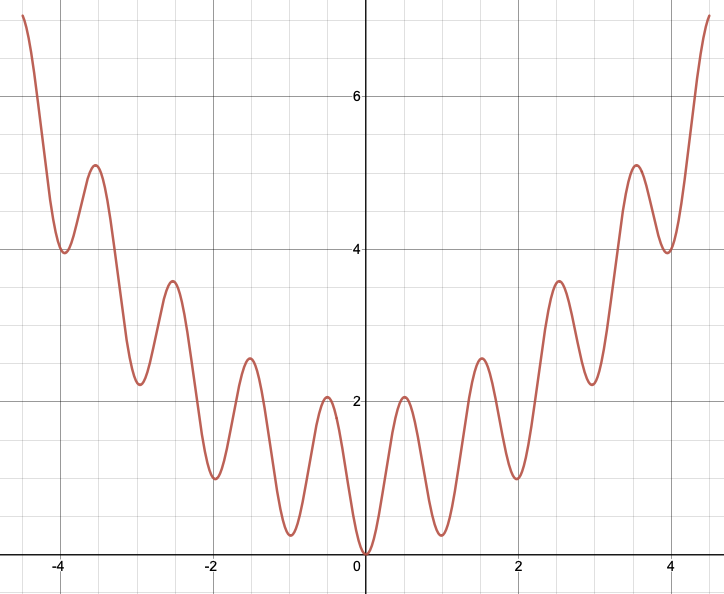
\includegraphics[width=0.5\linewidth]{a.png}
                \caption{Plot f(x)}
                \label{fig:enter-label}
            \end{figure}
            
        \item Find an initial point $x_0$ where gradient descent could end up converging to a local minimum that is not the global minimum.\\

            \begin{figure}[H]
                \centering
                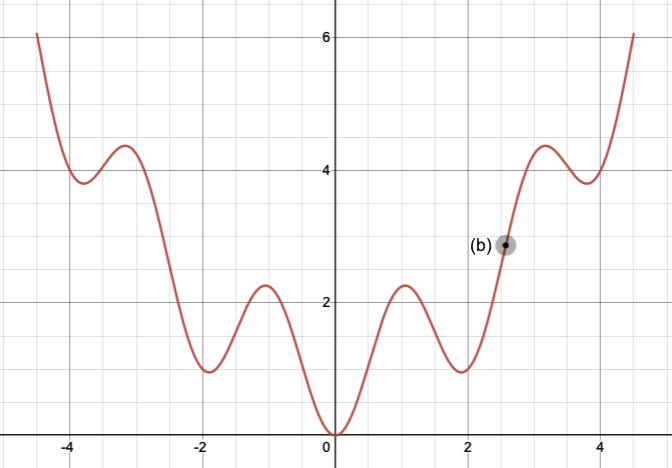
\includegraphics[width=0.5\linewidth]{b.png}
                \caption{Initial point $x_0 [3.15, 2.89]$}
                \label{fig:enter-label}
            \end{figure}

        \item Find a subset of $[−4.5, 4.5]$ such that $f(x)$ has a non-unique global minimum.\\ 
        
            \begin{figure}[H]
                \centering
                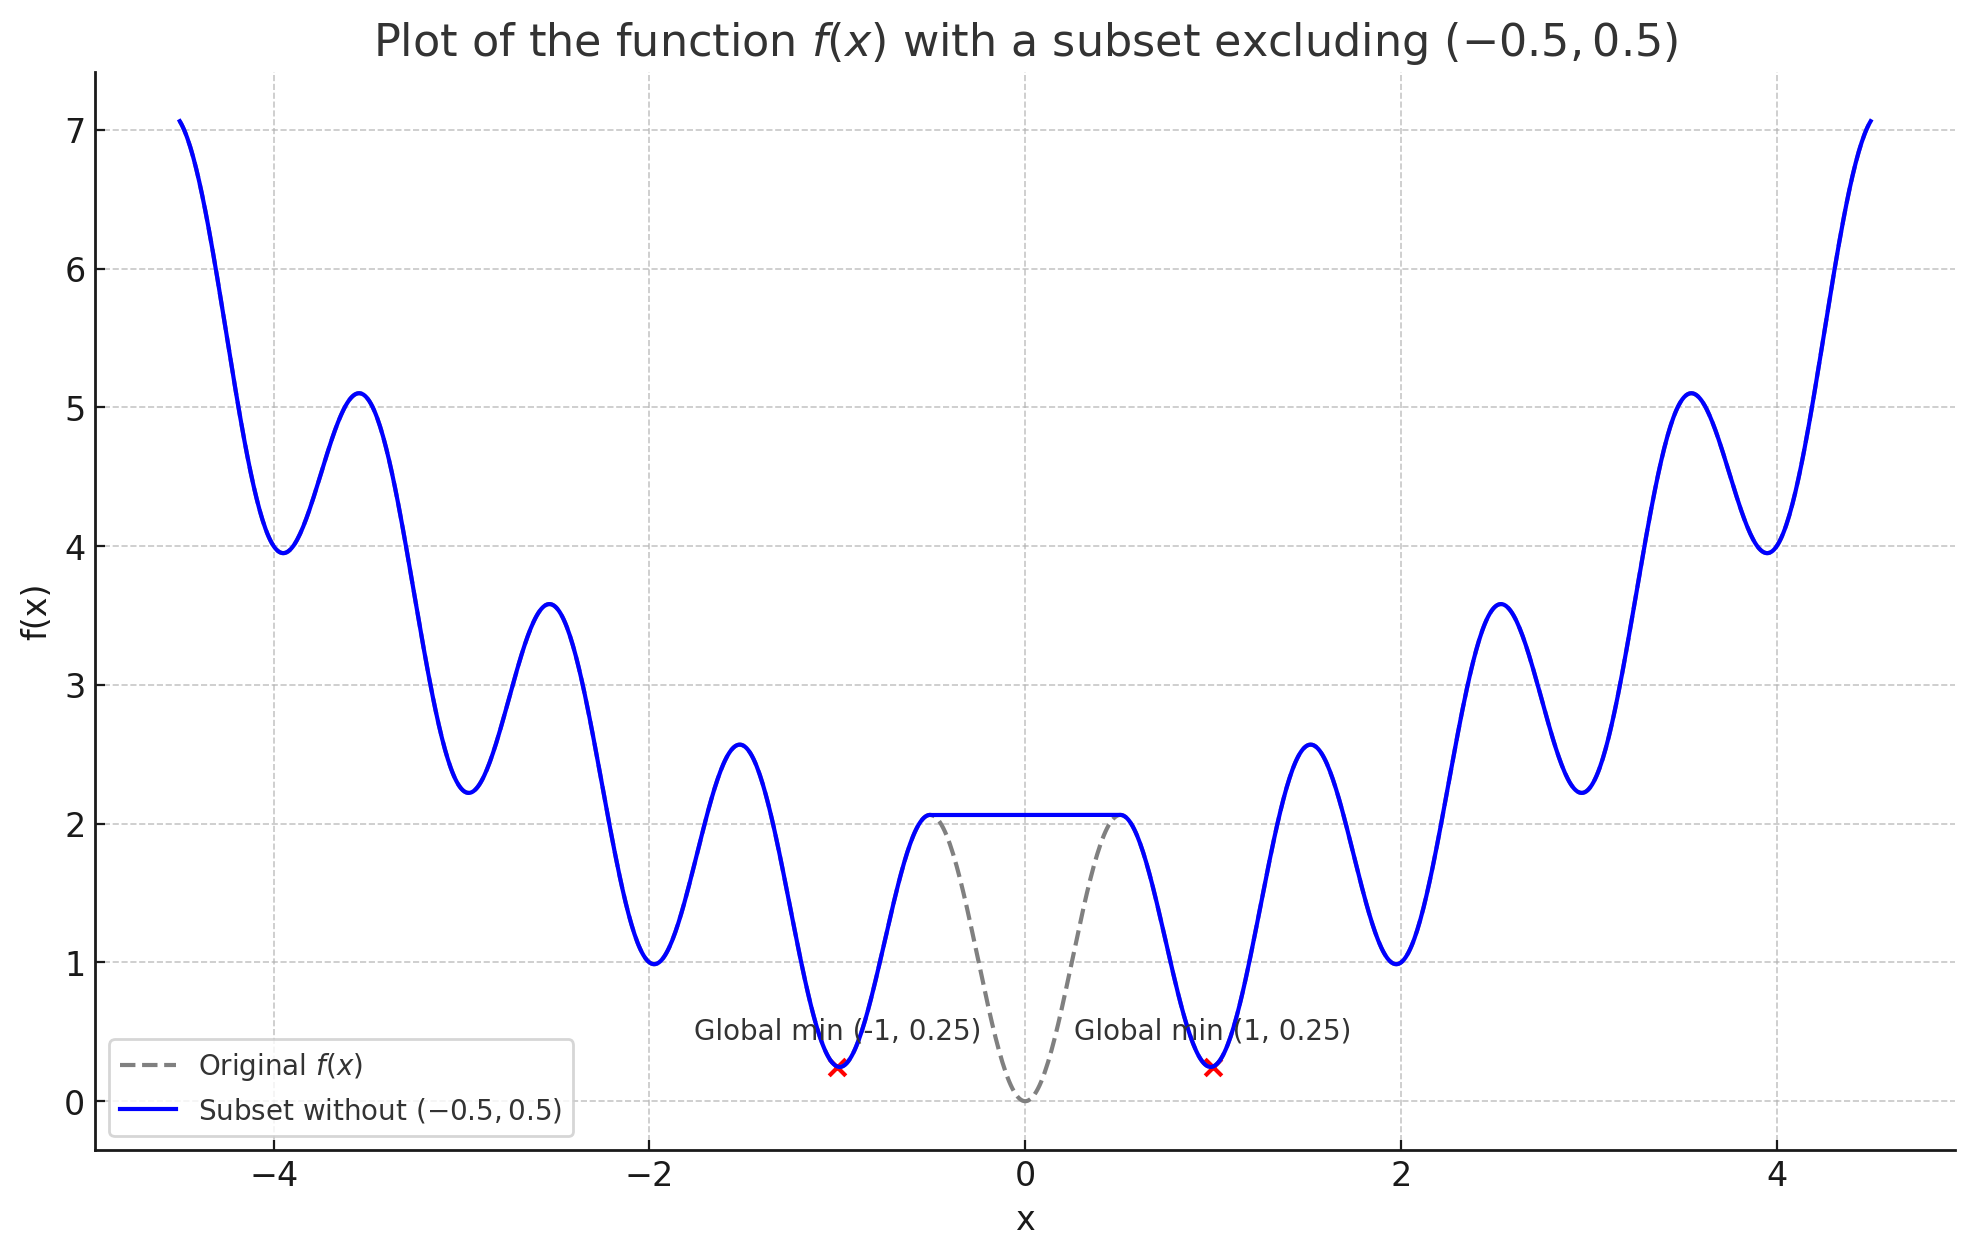
\includegraphics[width=0.5\linewidth]{c.png}
                \caption{Subset(c) = $\{ x \mid x \in [-4.5, -0.5] \cup [0.5, 4.5] \}$}
                \label{fig:enter-label}
            \end{figure}
    

        \item Find a subset of $[−4.5, 4.5]$ such that $f(x)$ has a unique global minimum.\\

        \begin{figure}[H]
            \centering
            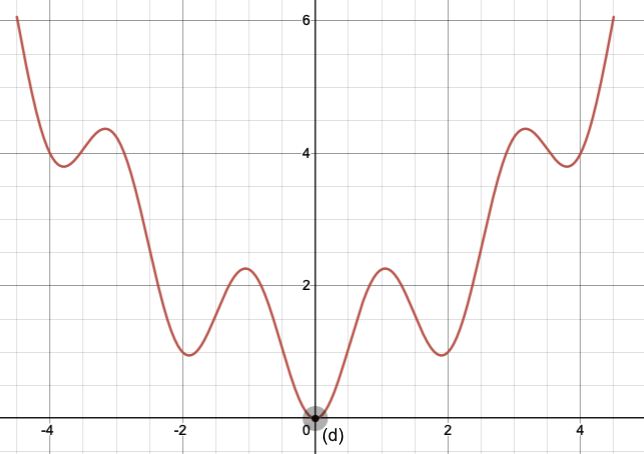
\includegraphics[width=0.5\linewidth]{d.png}
            \caption{Global Minimum Point [0,0]}
            \label{fig:enter-label}
        \end{figure}
    \end{enumerate}
\item Consider the linear regression problem in the previous lectures. Recall the “real estate" data set (see code on Canvas and more details in the slides). Consider the data set as it stands (i.e., incorporating all six x features and the target y being the house price of unit area). Given the candidate function\\ 

$y = w^Tx + b, w \in \R^6, b \in \R$, \\

and the cost function defined as RSS (unless noted otherwise), consider the following questions. Note the gradient formulation (if used) is expected to be derived analytically (then implemented in code), but the calculation of gradients can be done numerically in a variety of ways. As a result, your Python code is expected to use only standard Python libraries and numpy only.

\begin{enumerate}
    \item Starting from the initial point at$ ω = [1 1 1 1 1 1]^T$ and $b = 10$, execute the gradient descent algorithm for 4140 steps at a constant learning rate $\lambda = 0.001$, what is the updated solution (you are extremely likely to need some help from your computer here)?\\

    \begin{figure}[H]
        \centering
        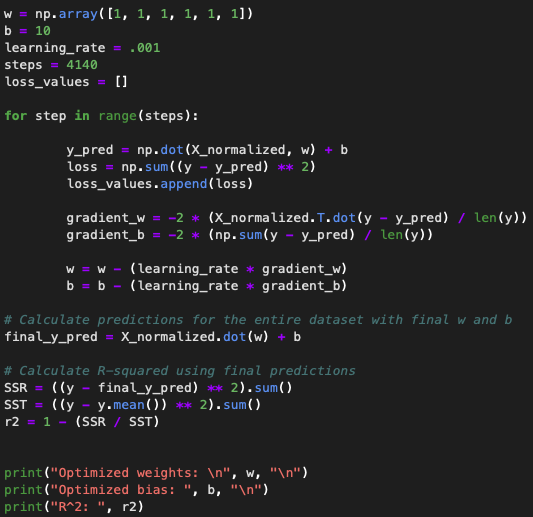
\includegraphics[width=0.5\linewidth]{2a.png}
        \caption{GD}
        \label{fig:enter-label}
    \end{figure}

    \textbf{The updated solution for GD is:} \\
    \textbf{Optimized weights: }\\
    X1 transaction date: $4.896591$\\
    X2 house age: $-2.170361$\\
    X3 distance to the nearest MRT station: $-5.584158$\\
    X4 number of convenience stores: $13.027288$\\
    X5 latitude: $10.220503$\\
    X6 longitude: $11.918416$\\

    \textbf{Optimized bias:} \\$19.688189362333627$ \\

    \textbf{Score:}\\
    $\R^2 \approx 0.4750$\\

    \textbf{Note: Please look for Python notebook sent with this report for code source.}\\

    \item If you follow the configuration described in the previous question (i.e., same initial point, same learning rate), for a sufficiently large running steps, will Gradient Descent lead you to the same optimal solution you have derived from the regression lecture (in other words, will it converge?)? Why?\\

    \begin{figure}[H]
        \centering
        \includegraphics[width=0.5\linewidth]{Unknown.png}
        \caption{Loss graph}
        \label{fig:enter-label}
    \end{figure}

    Yes, with a sufficiently large number of steps, gradient descent is expected to converge to a solution that is not the same but it is close to the optimal, as evidenced by the loss graph which shows a rapid initial decrease in cost and subsequent stabilization, indicating that the algorithm is approaching an optimal set of parameters.\\

    \textbf{Note: Please look for Python notebook sent with this report for code source.}\\

    \item Starting from the initial point at at $ω = [1 1 1 1 1 1]^T$ and $b = 10$, execute the stochastic gradient descent algorithm for 4140 steps at a constant learning rate $γ = 0.001$ (let’s say an invisible magical force is controlling the generation of all randomness on our planet, and your “stochastic" samples end up being the enumeration of the 414 points in the real estate data set following the exact order as it stands in the .csv file, thus to have the 4140 steps, you will have to repeat the enumeration at the same order for 10 times), what is the updated solution? Is your solution better than, the same with, or worth than the solution from 2(a)? Why?\\

    \begin{figure}[H]
        \centering
        \includegraphics[width=0.5\linewidth]{Screenshot 2024-02-29 at 8.42.34 AM.png}
        \caption{SGD}
        \label{fig:enter-label}
    \end{figure}

    \textbf{The updated solution for SGD is:} \\
    \textbf{Optimized weights: }\\
    X1 transaction date: $4.864761$\\
    X2 house age: $-2.178003$\\
    X3 distance to the nearest MRT station: $-5.602656$\\
    X4 number of convenience stores: $13.009351$\\
    X5 latitude: $10.227864$\\
    X6 longitude: $11.884743$\\

    \textbf{Optimized bias:} \\$19.620826963629238$ \\

    \textbf{Score:}\\
    $\R^2 \approx 0.4751$\\

    For 2(a), $R^2 \approx 0.4750 <  0.4751$. Hence, SGD was slightly better than GD.\\

    The slight improvement of SGD over GD in terms of $R^2$  can be attributed to SGD's ability to better navigate the cost function landscape through its frequent, varied updates, potentially finding a slightly more optimal set of parameters for the given dataset.\\
    
    \textbf{Note: Please look for Python notebook sent with this report for code source.}\\

    \item Let’s consider a cost that is not RSS, but takes the following form:\\
    $$J(X, y; w, b) = \sum^n_{i=1} |yi - w^t xi - b|$$

    \ i.\ Is the optimal solution unique? If the optimal solution is not unique, why? If it is unique, is it still the same with the original one derived from the RSS cost?\\

    The optimal solution is not necessarily unique because the absolute value makes the cost function piecewise linear, which can lead to multiple solutions that minimize the cost equally. \\

    \begin{figure}[H]
        \centering
        \includegraphics[width=0.5\linewidth]{Screenshot 2024-02-29 at 11.33.01 AM.png}
        \caption{Code for (1-5)}
        \label{fig:enter-label}
    \end{figure}

    \textbf{The updated solution for (1-5) is:} \\
    \textbf{Optimized weights: }\\
    X1 transaction date: $3.00745852$\\
    X2 house age: $2.48712785$\\
    X3 distance to the nearest MRT station: $1.47364676$\\
    X4 number of convenience stores: $2.6724$\\
    X5 latitude: $2.78491881$\\
    X6 longitude: $3.54698879$\\

    \textbf{Optimized bias:} \\$13.778$ \\

    \textbf{Score:}\\
    $\R^2 \approx -1.4247$\\

    \textbf{Note: Please look for Python notebook sent with this report for code source.}\\
    
    \ ii.\ For sufficiently large running steps with learning rate $\lambda = 0.001$, can you prove the convergence of Gradient Descent using the updated cost function (1-5)? Why?

    \begin{figure}[H]
        \centering
        \includegraphics[width=0.5\linewidth]{Unknown-1.png}
        \caption{(1-5)}
        \label{fig:enter-label}
    \end{figure}

    Based on the computation of the cost per iteration, I would say this model does not converge as the cost goes up and down, which indicates the algorithm is not being able to approach an optimal set of parameters.\\
\end{enumerate}
\end{enumerate}
\section{A ``Bonus" Question (1 pt)}
\noindent From a scale of 1 to 5, how difficult is HW3? 1 is ``I can do it in my sleep". 5 is ``Bowen is ridiculous". 0 is ``I refuse to answer this question". This is for my own reference to improve the quality of future assignments. Thanks!

\textbf{5 out of 5.}
    
\end{problem}

\end{document}